\documentclass[aspectratio=169]{beamer}
% SGSSS Beamer Preamble — shared across all lectures
% Brand colours from SGSSS logo

\usetheme{metropolis}

% --- Colour definitions ---
\definecolor{sgsssMagenta}{HTML}{A3217A}
\definecolor{sgsssGreen}{HTML}{2D6A3F}
\definecolor{sgsssBlack}{HTML}{1D1D1B}
\definecolor{sgsssWhite}{HTML}{FFFFFF}
\definecolor{sgsssLightGrey}{HTML}{F5F5F5}

% --- Metropolis colour overrides ---
\setbeamercolor{palette primary}{bg=sgsssMagenta, fg=sgsssWhite}
\setbeamercolor{title separator}{fg=sgsssGreen}
\setbeamercolor{progress bar}{fg=sgsssGreen, bg=sgsssLightGrey}
\setbeamercolor{frametitle}{bg=sgsssMagenta, fg=sgsssWhite}
\setbeamercolor{alerted text}{fg=sgsssMagenta}
\setbeamercolor{example text}{fg=sgsssGreen}
\setbeamercolor{block title}{bg=sgsssMagenta, fg=sgsssWhite}
\setbeamercolor{block body}{bg=sgsssLightGrey, fg=sgsssBlack}
\setbeamercolor{block title example}{bg=sgsssGreen, fg=sgsssWhite}
\setbeamercolor{block body example}{bg=sgsssLightGrey, fg=sgsssBlack}
\setbeamercolor{normal text}{fg=sgsssBlack}

% --- Fonts ---
\usepackage[T1]{fontenc}
\usepackage[sfdefault]{FiraSans}
\usepackage{FiraMono}
\setbeamerfont{frametitle}{size=\large}

% --- Packages ---
\usepackage{graphicx}
\usepackage{hyperref}
\usepackage{array}
\usepackage{booktabs}
\usepackage{minted}
\usepackage{fontawesome5}

% --- TikZ ---
\usepackage{tikz}
\usetikzlibrary{arrows.meta, positioning, shapes.geometric, trees, calc, decorations.pathmorphing, decorations.pathreplacing, fit, backgrounds}

% Reusable TikZ styles
\tikzset{
    server node/.style={rectangle, draw=sgsssGreen, fill=sgsssGreen!10, thick, minimum width=2.5cm, minimum height=1.2cm, align=center, font=\small},
    client node/.style={rectangle, draw=sgsssMagenta, fill=sgsssMagenta!10, thick, minimum width=2.5cm, minimum height=1.2cm, align=center, font=\small},
    api node/.style={rectangle, draw=sgsssGreen, fill=sgsssGreen!15, thick, rounded corners, minimum width=2.5cm, minimum height=1.2cm, align=center, font=\small},
    data node/.style={rectangle, draw=sgsssBlack, fill=sgsssLightGrey, thick, minimum width=2cm, minimum height=1cm, align=center, font=\small},
    arrow style/.style={-{Stealth[length=3mm]}, thick, sgsssBlack},
    html tag/.style={rectangle, draw=sgsssMagenta, fill=sgsssMagenta!8, rounded corners=2pt, font=\ttfamily\small, inner sep=4pt},
    json key/.style={rectangle, draw=sgsssGreen, fill=sgsssGreen!8, rounded corners=2pt, font=\ttfamily\small, inner sep=4pt},
}

% --- Minted configuration ---
\setminted{
    fontsize=\footnotesize,
    frame=leftline,
    framesep=2mm,
    baselinestretch=1.1,
    bgcolor=sgsssLightGrey,
    breaklines,
    linenos=false,
}
\setminted[python]{style=friendly}
\setminted[r]{style=friendly}

% --- Convenience commands ---
\newcommand{\pythoncode}[1]{\mintinline{python}{#1}}
\newcommand{\rcode}[1]{\mintinline{r}{#1}}
\newcommand{\httpstatus}[2]{\texttt{#1} \textit{#2}}

% --- Footer (page numbers only; logo on title slide only) ---
\setbeamertemplate{frame footer}{%
    \insertframenumber/\inserttotalframenumber%
}

% --- Metadata ---
\author{Dr Diarmuid McDonnell}
\institute{Braw Data Ltd \and Gradel Institute of Charity, University of Oxford}
\date{24 February 2026}


\title{LLMs as Coding Assistants}
\subtitle{SGSSS --- Collecting Digital Data}

\begin{document}

% -------------------------------------------------------
% Slide 1: Title
% -------------------------------------------------------
{
\setbeamertemplate{frame footer}{}
\begin{frame}[plain]
    \begin{center}
        \includegraphics[height=2.5cm]{../img/SGSSS_Stacked.png}\\[0.8cm]
        {\Large\bfseries\color{sgsssMagenta} Collecting Digital Data}\\[0.2cm]
        {\large LLMs as Coding Assistants}\\[0.6cm]
        {\normalsize Dr Diarmuid McDonnell}\\[0.1cm]
        {\small Braw Data Ltd \(\cdot\) Gradel Institute of Charity, University of Oxford}\\[0.3cm]
        {\small 24 February 2026}
    \end{center}
\end{frame}
}

% -------------------------------------------------------
% Slide 2: Section title
% -------------------------------------------------------
\section{LLMs as Coding Assistants}

% -------------------------------------------------------
% Slide 2: What are LLMs?
% -------------------------------------------------------
\begin{frame}{What Are LLMs?}
    A \textbf{Large Language Model} is a statistical model trained on vast amounts of text and code.

    \vspace{0.2cm}
    \begin{center}
    \scalebox{0.85}{%
    \begin{tikzpicture}[node distance=2.2cm]
        % Training data node
        \node[data node, minimum width=2.2cm] (data) {%
            \faIcon{book} Books\\
            \faIcon{code} Code\\
            \faIcon{globe} Web pages};

        % Model node
        \node[api node, right=of data, minimum width=2.2cm, minimum height=1.2cm] (model) {%
            \faIcon{brain}\\LLM};

        % Prompt node
        \node[client node, above right=0.6cm and 2.2cm of model, minimum width=2.2cm] (prompt) {%
            \faIcon{keyboard}\\Prompt};

        % Response node
        \node[server node, below right=0.6cm and 2.2cm of model, minimum width=2.2cm] (response) {%
            \faIcon{comment-dots}\\Response};

        % Arrows
        \draw[arrow style] (data) -- (model) node[midway, above, font=\small] {Training};
        \draw[arrow style] (prompt) -- (model) node[midway, above, font=\small, sloped] {Input};
        \draw[arrow style] (model) -- (response) node[midway, above, font=\small, sloped] {Output};
    \end{tikzpicture}}
    \end{center}

    \vspace{0.1cm}
    {\small You provide a \textbf{prompt} (a question or instruction), and the model generates a \textbf{response}.}
\end{frame}

% -------------------------------------------------------
% Slide 3: Paid vs open models
% -------------------------------------------------------
\begin{frame}{Paid vs Open Models}
    \begin{center}
    \begin{tabular}{@{}p{5.5cm}p{5.5cm}@{}}
        \toprule
        \textbf{Paid (ChatGPT, Claude)} & \textbf{Open (Llama, Mistral)} \\
        \midrule
        Hosted by provider & Run locally or self-host \\[0.15cm]
        Subscription / API fees & Free to use \\[0.15cm]
        Often more capable & Improving rapidly \\[0.15cm]
        Data sent to provider & Data stays with you \\[0.15cm]
        Easy to use (chat UI) & Requires some setup \\
        \bottomrule
    \end{tabular}
    \end{center}

    \vspace{0.4cm}
    \begin{exampleblock}{Tip}
        For this course, any chat-based LLM will work --- use whichever you have access to.
    \end{exampleblock}
\end{frame}

% -------------------------------------------------------
% Slide 4: How to prompt for code
% -------------------------------------------------------
\begin{frame}{How to Prompt for Code}
    \small
    \begin{exampleblock}{\faIcon{check-circle} Good prompt}
        ``Write a Python script using \texttt{requests} to download stop-and-search data from the UK Police API for the City of London force. Save the results as a JSON file.''
    \end{exampleblock}

    \vspace{0.15cm}

    \begin{alertblock}{\faIcon{times-circle} Bad prompt}
        ``Get me some police data.''
    \end{alertblock}

    \vspace{0.2cm}
    \textbf{What makes a good prompt?}
    \begin{itemize}\itemsep0.05cm
        \item Specify the \textbf{programming language} and \textbf{libraries}
        \item Provide the \textbf{exact URL} or API endpoint
        \item State the \textbf{desired output} format
        \item Include relevant \textbf{parameters} (e.g., force name, date range)
    \end{itemize}
\end{frame}

% -------------------------------------------------------
% Slide 5: What LLMs are good at
% -------------------------------------------------------
\begin{frame}{What LLMs Are Good At}
    \small
    \begin{itemize}\itemsep0.05cm
        \item[\textcolor{sgsssGreen}{\faIcon{check-circle}}] \textbf{Boilerplate code} --- standard request/response patterns, file I/O, data wrangling
        \item[\textcolor{sgsssGreen}{\faIcon{check-circle}}] \textbf{Syntax and library usage} --- ``How do I use \texttt{pandas.json\_normalize}?''
        \item[\textcolor{sgsssGreen}{\faIcon{check-circle}}] \textbf{Explaining error messages} --- paste a traceback and ask what went wrong
        \item[\textcolor{sgsssGreen}{\faIcon{check-circle}}] \textbf{Converting between languages} --- turn a Python script into R (or vice versa)
        \item[\textcolor{sgsssGreen}{\faIcon{check-circle}}] \textbf{Generating documentation} --- docstrings, comments, README files
    \end{itemize}

    \vspace{0.15cm}
    \begin{exampleblock}{Key insight}
        LLMs excel at tasks that are \textbf{well-documented} and \textbf{widely practised} online.
    \end{exampleblock}
\end{frame}

% -------------------------------------------------------
% Slide 6: What LLMs are bad at
% -------------------------------------------------------
\begin{frame}{What LLMs Are Bad At}
    \begin{itemize}
        \item[\textcolor{sgsssMagenta}{\faIcon{times-circle}}] \textbf{Up-to-date API endpoints/parameters} --- training data has a cut-off date
        \item[\textcolor{sgsssMagenta}{\faIcon{times-circle}}] \textbf{Complex multi-step logic} --- long workflows with many dependencies
        \item[\textcolor{sgsssMagenta}{\faIcon{times-circle}}] \textbf{Understanding your specific research context} --- it doesn't know your data
        \item[\textcolor{sgsssMagenta}{\faIcon{times-circle}}] \textbf{Guaranteeing correctness} --- output looks plausible but may be wrong
        \item[\textcolor{sgsssMagenta}{\faIcon{times-circle}}] \textbf{Hallucinated function names} --- confidently invents functions that don't exist
    \end{itemize}

    \vspace{0.4cm}
    \begin{alertblock}{Remember}
        LLMs are \textbf{confident}, not \textbf{correct}. Always verify their output.
    \end{alertblock}
\end{frame}

% -------------------------------------------------------
% Slide 7: Critical evaluation
% -------------------------------------------------------
\begin{frame}{Critical Evaluation of LLM-Generated Code}
    \begin{alertblock}{Golden rule}
        You \textbf{must} understand the code yourself. If you can't explain what it does, don't use it.
    \end{alertblock}

    \vspace{0.3cm}
    \begin{itemize}
        \item \faIcon{vial} \textbf{Always test} LLM-generated code --- run it, inspect the output
        \item \faIcon{book-open} \textbf{Check API docs} match what the LLM suggests --- endpoints, parameters, authentication
        \item \faIcon{ghost} \textbf{Be wary of hallucinated libraries/functions} --- verify they actually exist
        \item \faIcon{sync-alt} \textbf{Consider reproducibility} --- LLM outputs vary between sessions and models
        \item \faIcon{lock} \textbf{Security risks} --- never paste API keys, passwords, or sensitive data into a chat
    \end{itemize}
\end{frame}

% -------------------------------------------------------
% Slide 8: Next up
% -------------------------------------------------------
\begin{frame}{Next Up}
    \begin{center}
        {\Large \alert{Practical 4: LLM Showdown}}\\[0.5cm]
        \begin{itemize}
            \item Compare different LLMs on the same coding task
            \item Evaluate the quality, correctness, and usability of generated code
            \item Apply the critical evaluation criteria from this lecture
        \end{itemize}
        \vspace{0.5cm}
        {\normalsize Use your preferred LLM (ChatGPT, Claude, Llama, etc.)\\to complete the challenge tasks.}
    \end{center}
\end{frame}

% -------------------------------------------------------
% Slide 9: Thank you and resources
% -------------------------------------------------------
\begin{frame}{Thank You!}
    \centering
    \textbf{Dr Diarmuid McDonnell}\\[0.15cm]
    {\small Director, Braw Data Ltd}\\
    {\small Visiting Fellow, Gradel Institute of Charity, University of Oxford}\\[0.3cm]

    {\footnotesize \faIcon{globe}\;\; \href{https://www.brawdata.co.uk}{www.brawdata.co.uk} \quad
    \faIcon{university}\;\; \href{https://www.gradelinstituteofcharity.co.uk/diarmuid-mcdonnell}{Gradel Institute of Charity} \quad
    \faIcon{github}\;\; Course materials on GitHub}\\[0.4cm]

    \includegraphics[height=2.5cm]{../img/SGSSS_Stacked.png}\\[0.4cm]

    {\small Thank you for attending the \textbf{SGSSS Collecting Digital Data} course.\\Good luck with your research!}
\end{frame}

\end{document}
